\chapter{Familiarisation avec �quipements et exp�riences pr�liminaires}
\label{s:Familiarisation_Experiences}


\section{Structure m�canique}
\label{s:Structure_mecanique}


La base m�canique du robot est assur�e par les diff�rentes plate-formes et tiges filet�es fournies pour le projet, il en revient donc � nous de d�cider de l'agencement de ces composantes afin de produire un robot m�caniquement efficace. De mani�re � bien mod�liser le robot et ainsi faciliter l'installation de futurs �quipements, il fut d�cid� de r�aliser une repr�sentation 3D du prototype. La figure \ref{f:CAD} pr�sente le dessin ainsi r�alis�, bien que grossier il fut construit � partir de mesures exactes effectu�es sur le robot. Ce dessin est tr�s utile pour planifier d'avance l'emplacement des diff�rents syst�mes qui seront ajout�s au cours du projet en plus de permettre une meilleure planification de l'�lectrique autant au niveau des fils que des circuits. 

\medbreak

On peut remarquer que sur ce dessin l'ordinateur embarqu� est situ� sur la plate-forme centrale, ce choix est justifi� par le fait que nous d�sirons avoir l'�lectronique le plus proche possible des moteurs DC afin de limiter la longueur des fils. La batterie LiPO repr�sent�e par le bloc bleu est positionner sur la plate-forme la plus basse de mani�re � assurer un centre de gravit� assez bas. Le bloc jaune repr�sente environ les dimensions de l'�lectronique pr�sente sur cet �tage du robot. Bien �videmment, toutes ces composantes seront fix�es en place. Bien que le pont en H n'est pas observable sur cette image il est important de noter que celui-ci peu �tre fix� sous la base en cas de besoin. Le pr�henseur pr�sent� � la section \ref{s:Prehenseur} est repr�sent� sur le devant du robot, la cam�ra embarqu�e est install�e directement au-dessus de ce dispositif sur l'�tage le plus haut. L'utilisation de ce dessin 3D et d'un autre dessin de la borne de rechargement a aussi permis de mesurer, sans faire de prototype de pr�henseur, la hauteur ad�quate de la bobine de chargement du condensateur afin de bien aligner les deux dispositifs.



\begin{figure}[htp]
   \centering
   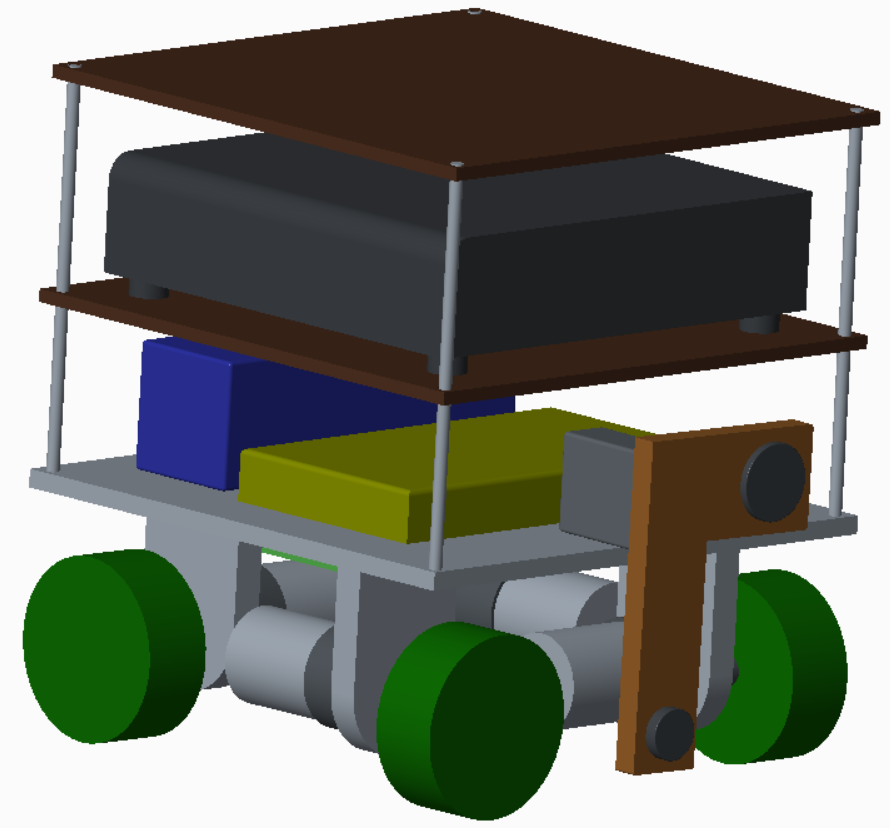
\includegraphics[width=0.95\textwidth]{fig/ROBOT.png}
   \caption{Repr�sentation 3D du robot}
   \label{f:CAD}
\end{figure}

\pagebreak

\section{Syst�me de pr�henseur et d'�lectroaimant}
\label{s:Prehenseur}

Afin de rendre le pr�henseur le plus simple possible m�caniquement, nous choisissons de le faire en forme d'�querre. Aux deux extr�mit�s de l'�querre sont situ�s l'�lectroaimant et le secondaire du transformateur qui permet de charger le condensateur d'alimentation de l'�lectroaimant. Il devient donc tr�s ais� d'enligner le syst�me de recharge avec la station de recharge ainsi que de soulever les tr�sors en faisant tourner l'�querre de 90 degr�s dans un sens ou dans l'autre. Cette rotation est assur�e par un servomoteur situ� au centre de l'�querre. La figure \ref{f:CAD} permet de comprendre facilement la m�canique du pr�henseur. Le dessin 3D permet donc de se faire une bonne id�e des dimensions du bras du pr�henseur de mani�re � ce qu'il soit efficace. Un servomoteur pr�sentant suffisamment de couple ($6.4Kg\cdot cm$ � 6V) permet d'actionner le pr�henseur.

\medbreak

L'�lectroaimant est un mod�le pr�-fait achet� en ligne. Il s'agit du mod�le \textit{Grove} de la compagnie \textit{seeed} (voir section \ref{liste_pieces}). Cet aimant peut soulever une charge de 1kg pour un courant de 400mA. En assumant que la force g�n�r�e par l'aimant d�pend quadratiquement du courant le parcourant et en sachant que le poids des tr�sors est de 30g l'unit�, on estime le courant n�cessaire pour soulever les tr�sors autour de 5mA. Pour avoir une marge de s�curit� ainsi que de pouvoir attirer les tr�sors <<� distance>>, on augmente ce courant � 20mA. Le courant dans l'�lectroaimant est contr�l� par une source de courant � diode Zener (voir figure \ref{f:source_courant}).

\medbreak

L'�nergie n�cessaire pour soulever un tr�sor pendant 10 minutes par l'�lectroaimant est de 60J ($U = 5V \times 20mA \times 10min \times 60s / min$). Un condensateur de 0.5F � 5V contient 62.5J d'�nergie ($U = 0.5 \times C \times V^2$). C'est donc cette valeur de condensateur qui est choisie pour aliment� l'�lectroaimant.

\medbreak

Afin de permettre de faire des tests ainsi que de s'assurer un degr� de s�ret�, un condensateur de 1F est �galement consid�r� dans le design de ce syst�me.

\begin{figure}[htp]
	\centering
	
\includegraphics[scale = 0.25]{fig/source_courant.png}
	\caption{Source courant � diode Zener}
	\label{f:source_courant}
\end{figure}


\pagebreak

\section{Station de recharge}
\label{s:Station_recharge}



\section{Contr�le des moteurs}
\label{s:Controle_moteurs}

Afin de commander les moteurs du robot, il est n�cessaire d'avoir une routine d'asservissement. Afin de communiquer les commandes avec les moteurs DC, l'Arduino Mega est choisi. Celui-ci poss�de une vitesse d'horloge de 16 MHz et 256kB de m�moire flash pour 45\$ \cite{MEG00}, ce qui est un bon �quilibre performance/prix pour les besoins du projet.
\medbreak
Les moteurs utilis�s pour entra�ner les roues du robot poss�dent 6400 valeurs de position par rotation. Si une interruption est effectu�e � chaque modification de cette valeur, on risque d'emp�cher l'ex�cution compl�te d'une boucle d'asservissement entre deux interruptions. Donc, si une interruption est lev�e � chaque modification de la position, il faut s'assurer que le calcul de la vitesse de rotation se fasse apr�s un nombre multiple d'interruptions, avec un compteur de temps.
\medbreak
Pour ce qui a trait � la communication avec les moteurs DC, un shield Adafruit se connectant directement sur l'Arduino Mega est utilis�. Avec celui-ci, il est possible de g�n�rer des ondes modul�es (PWM) servant � contr�ler les quatres roues individuellement, avec chacun une r�solution de 8 bits et jusqu'� 1.2 amp�res par canal\cite{SLD00}. Cette division de la commande est utile lors d'un d�placement en diagonale, et pourrait �galement �tre utile pour continuer le fonctionnement dans le cas d'une roue d�fectueuse. Ce dispositif est utilis� pour contr�ler les moteurs pour les premiers tests, bien �videmment l'utilisation du pont en H fournit fera aussi l'objet de tests.
\medbreak
En r�sum�, l'ordinateur envoie des instructions de direction au microcontr�leur Arduino, qui ex�cute alors une routine de d�placement. Celle-ci est bas�e sur un asservissement de vitesse, d�termin�e par des interruptions lors de la rotation des servomoteurs. Les commandes de l'Arduino sont alors communiqu�es aux roues � l'aide d'un shield Adafruit permettant de leur d�livrer de la puissance.



\section{Localisation du robot et des �les}
\label{s:Localisation_Robot_Iles}

La cam�ra Logitech C905 situ� en hauteur permet de visionner une grande partie de la table. Celle-ci sera branch� USB � la station de base. Les tests effectu� jusqu'� pr�sent nous on permis de contempler la vision limiter de la table de jeux (figure \ref{f:testCameraMonde}). C'est donc pour cette raison que seul une premi�re approximation sur la position des tr�sors pourra �tre faite. La localisation plus pr�cise de ceux-ci se fera par la cam�ra embarqu� (idem pour la station de recharge). Voir la section \ref{s:Reperage}.
\medbreak
La d�tection des �les et du robot se fait par la station de base � l'aide de la cam�ra monde. Pour ce faire, le logiciel OpenCV est utilis�. Premi�rement, l'image est d�coup� de sorte � ce qu'elle ne contienne que la table de jeux. Cet outil tr�s puissant nous permet aussi de d�tecter les contours d'objet � l'int�rieur d'image en utilisant les couleur pour les distinguer (BGR). Les contours jaune, bleu, rouge et vert sont d�tect� afin de rep�rer les �les. Afin d'�viter les erreurs, une relation entre le nombre de coin, le p�rim�tre et l'air des contours sera v�rifi�. La validation de cette relation confirmera la pr�sence d'une �le tout en indiquant sa forme et sa couleur (selon le nombre de coin et l�intervalle BGR utilis�). Nous avons d�j� test� ces �tapes et elle semble plut�t efficace (figure \ref{f:testDetectionCouleur}). Pour localiser le robot, une forme et couleur particuli�re sera plac� au dessus du robot. On proc�dera de fa�on similaire pour le d�tecter.


\section{Rep�rage des tr�sors et de la station de recharge}
\label{s:Reperage}

La cam�ra Logitech C905 situ�e sur le robot permettra de rep�rer les diff�rents tr�sors ainsi que la station de recharge. Cette cam�ra sera contr�l�e par les Servomoteurs fournis qui permettront � la cam�ra un d�placement sur son axe horizontal et vertical afin d'augmenter le champ de vision du robot. Afin de contr�ler le � Polulu � Maestro 6-Channel USB Servo Controller, des commandes seront envoy�es par USB � partir de l'ordinateur embarqu� situ� sur le robot. La cam�ra embarqu�e sera �galement reli�e directement � l'ordinateur embarqu�e afin d'�tre aliment�e et de fournir les images capt�es. La fr�quence de captation des images reste � d�terminer puisqu'il faudra d�cider � quel intervalle nous devons mettre � jour la vision du robot. L'envoi des commandes afin de contr�ler la prise d'image par la cam�ra sera effectu�e par la librairie Pygame en Python.

Afin de d�tecter les tr�sors, une premi�re approximation de leur position est effectu�e par la cam�ra monde qui, � l'aide de la librairie cv2 de OpenCV, permet de localiser dans une image un intervalle de couleur BGR. Le choix de la librairie d'OpenCV est justifi� par le fait qu'elle poss�de toutes les fonctions n�cessaires � un programme de vision complet et qu'elle s'int�gre facilement au reste du code en Python. Les tests effectu�es avec la cam�ra monde ont permis de venir � la conclusion que la d�tection des tr�sors s'effectuent tr�s bien. Par contre, les tests ont �galement permis de constater que la cam�ra monde ne voit pas le fond de la table et donc, certains tr�sors ne seront pas d�tecter par la cam�ra monde, justifiant la d�tection des tr�sors �galement par la cam�ra embarqu�e. Par la suite, les diff�rents pixels correspondant � la couleur des tr�sors sont plac�s dans un masque des tr�sors. Gr�ce � la position relative de ces points dans le masque des tr�sors, il est possible d'avoir une position approximative de ces tr�sors dans la carte virtuelle. Afin de confirmer la d�tection de ces tr�sors ou pour rep�rer les tr�sors qui seront hors du champ de vision du robot, la m�me op�ration de d�tection des couleurs est effectu�e ensuite par la cam�ra embarqu�e autour des coordonn�es approximative d�tect�e par la cam�ra monde.

La station de recharge, quant � elle, est marqu�e d'une couleur caract�ristique lui permettant de se distinguer du reste du d�cor. Comme la position et l'orientation du robot est connue en tout temps et que la station de recharge est toujours situ� au m�me endroit, la d�tection de celle-ci est assez simple. Comme le robot peut �tre plac� � n'importe quel endroit au d�part sur la table, la cam�ra monde est charg�e � l'initialisation du programme de d�tecter la position et l'orientation de celui-ci. Afin de r�aliser cette t�che, un drapeau pirate est plac� sur le dessus du robot afin d'indiquer l'orientation ainsi que la position de celui-ci et sera d�tecter par notre programme de vision.




\section{Alimentation du robot}
\label{s:Alimentation}

Pour alimenter ad�quatement tous les syst�mes pr�sents sur le robot, on doit avoir une batterie avec un voltage qui se situe entre 21V et 30V pour alimenter le r�gulateur de l'ordinateur embarqu�, qui fonctionne � 19V avec un courant de 3.5A. On doit �galement avoir assez de puissance pour que les moteurs et l'�lectronique de contr�le puissent fonctionner pendant au moins dix minutes. La puissance dont le robot a besoin se d�finit surtout par celle des moteurs, des servomoteurs et de l'ordinateur embarqu�. Les moteurs demandent au maximum 800mA � 12V lorsque le rotor est compl�tement bloqu� et les servomoteurs qui servent � contr�ler la cam�ra demandent environ 30mA � 5V lorsqu'ils sont sollicit�s, soit un court instant. On utilise �galement un servomoteur plus puissant pour d�placer le pr�henseur, celui-ci risque de consommer plus de puissance � cause de l'effort plus important qui sera fourni. En additionnant la puissance de ces syst�mes, la puissance requise est d'environ 110W dans le pire des cas. Nous avons donc choisi une batterie LiPO 6S de 4 500mA, ce qui peut donner 27A, pour un total de 599W en 10 minutes. Les six cellules sont n�cessaires pour avoir 22.2V, ce qui permet d'obtenir le 19V requis pour l'ordinateur embarqu�. Le 4 500mA est justifi�, car on veut pouvoir travailler sur le robot plus longtemps que 10 minutes � des fins de test. Nous avons calcul� que cette batterie pourrait nous donner environ 50 minutes d'autonomie. 
\bigbreak
L'utilisation d'une batterie LiPO n�cessite un chargeur intelligent qui refuse de charger la batterie si les cellules ont un voltage trop faible, car la batterie pourrait exploser. Nous avons donc achet� un tel chargeur et on utilise �galement un sac de protection pour diminuer l'impact d'une �ventuelle explosion. L'utilisation d'une LiPO requi�re �galement un syst�me qui d�clenche une alarme sonore lorsqu'il faut recharger la batterie, pour justement emp�cher les risques d'explosions. Cette fonction est assur�e par un petit afficheur de tension, con�u sp�cialement pour les batteries LiPO, qui sonne quand la tension des cellules est trop faible. 
\bigbreak
Le robot a donc besoin de trois niveaux de tension diff�rents pour fonctionner. On utilise des r�gulateurs DC-DC pour avoir une tension stable, aux tensions d�sir�es. Le r�gulateur de l'ordinateur embarqu� est fourni. Pour le 12V et le 5V, nous avons choisi de prendre trois fois le m�me r�gulateur, qui prend 4V � 38V en entr�e et peut fournir 1.25V � 36V en sortie. Il y aura donc deux r�gulateur pour le 12V, pour s�parer l'alimentation des moteurs et celle du Arduino, et un r�gulateur pour le 5V. Ce r�gulateur peut fournir un maximum 5A et il est dot� d'un afficheur de tension pour conna�tre facilement le niveau de tension en sortie. On prot�ge nos syst�mes avec des fusibles pour s'assurer de ne rien briser. On a choisi de prendre un fusible de 10A directement � la sortie de la batterie pour prot�ger l'ensemble du syst�me. Pour les moteurs, on utilise un fusible de 5V, ensuite un fusible de 2A pour l'alimentation de l'Arduino et enfin un fusible de 3A pour les circuits �lectroniques du 5V. Un interrupteur situ� directement suite � la batterie permet finalement d'actionner l'ensemble du syst�me. La figure \ref{f:alim} pr�sente un diagramme en bloc de l'alimentation.

\begin{figure}[htp]
   \centering
   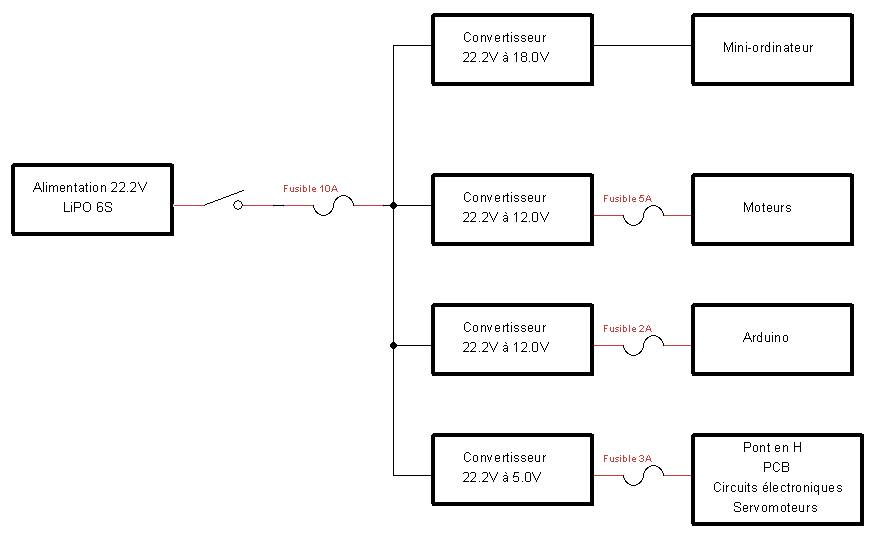
\includegraphics[width=1\textwidth]{fig/alim.jpg}
   \caption{Diagramme en bloc de l'alimentation}
   \label{f:alim}
\end{figure}


\section{Transmission du code Manchester}
\label{s:Communication}

La transmission sans-fil du code Manchester est assur�e par une combinaison LED-photor�cepteur. La LED est situ�e sur le dessus de la station de recharge et le photor�cepteur est situ� sur le dessus du robot. Ce syst�me de communication sans-fil est limit� � des distances relativement faibles, mais le robot �tant en contact physique avec la station de recharge, cette contrainte ne pose pas de probl�me. Le dessin 3D pr�sent� pr�c�demment servira � planifier la disposition exacte de ces composantes une fois les pi�ces re�ues et le concept test� de mani�re � minimiser les temps de construction et d'assemblage.

\medbreak

La LED est modul� par un microcontr�leur situ� sur la station de recharge. Le mod�le du microcontr�leur reste � d�terminer, mais devra �tre assez simple et peu co�teux puisque sa t�che sera relativement simple. Ce syst�me de communication est illustr� sur le sch�ma \ref{f:led_robot}.

\medbreak

Le document \cite{COM00} explique bri�vement comment r�aliser un tel syst�me et est utilis� comme r�f�rence pour r�aliser notre syst�me.


\begin{figure}[htp]
	\centering
	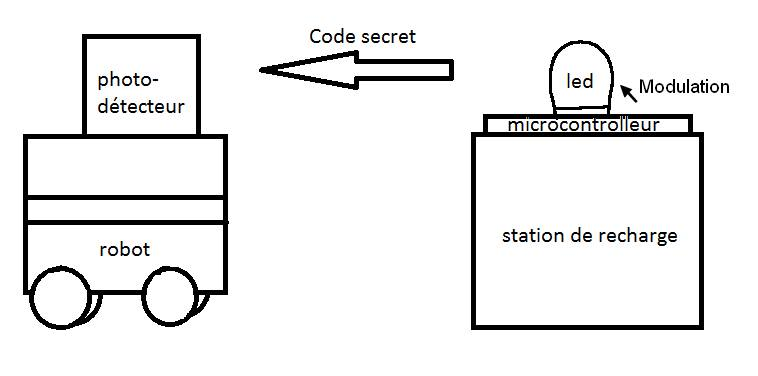
\includegraphics[scale = 0.4]{fig/led_robot.png}
	\caption{Communication sans-fil entre la station de recharge et le robot}
	\label{f:led_robot}
\end{figure}

\section{Liste des pi�ces achet�es}

\begin{description}
\label{liste_pieces}
	\item[Buck (x3)] \url{http://www.ebay.ca/itm/171445007919?_trksid=p2050601.m570.l6004&_trkparms=gh1g\%3DI171445007919.N41.S2.R2.TR2}
	\item[Batterie LiPo] \url{http://www.hobbyking.com/hobbyking/store/__10284__Turnigy_4500mAh_6S_30C_Lipo_Pack.html}
	\item[Chargeur de batterie LiPO] \url{http://www.hobbyking.com/hobbyking/store/__40270__Hobbyking_8482_T682_AC_6s_10A_90W_Eco_Touch_Balance_Charger_Discharger.html}
	\item[Alarme batterie] \url{http://www.hobbyking.com/hobbyking/store/__74024__HobbyKing_8482_Lipo_Voltage_Checker_2S_8S_.html}
	\item[Arduino Mega] \url{http://www.robotshop.com/ca/en/arduino-mega-2560-microcontroller-rev3.html}
	\item[Servomoteur de contr�le du pr�henseur] \url{http://www.robotshop.com/ca/en/hitec-hs-485hb-servo-motor.html}
	\item[Shield pour <<driver>> les moteurs] \url{http://www.robotshop.com/ca/en/motor-shield-kit-arduino-v2.html}
	\item[�lectroaimant \textit{Grove}] \url{http://www.seeedstudio.com/wiki/Grove_-_Electromagnet}
\end{description}
	

%Autres sections au choix selon ce qui sera d�cid�